\documentclass[11pt,a4paper]{article}
\usepackage[margin=2.3cm]{geometry}
\usepackage{amsmath,amssymb}
\usepackage{graphicx}
\usepackage{booktabs}
\usepackage{xcolor}
\usepackage[colorlinks=true,linkcolor=blue!50!black,citecolor=blue!50!black,urlcolor=blue!50!black]{hyperref}
\usepackage{natbib}
\graphicspath{{../plots/}}

\newcommand{\scrit}{\Sigma_{\rm crit}}
\newcommand{\msun}{\mathrm{M}_\odot}
\newcommand{\arcsecond}{^{\prime\prime}}
\newcommand{\kms}{\,{\rm km\,s^{-1}}}

\title{Which galaxies make sub-arcsecond quasar lenses?}
\author{Working note for the QUELLS introduction}
\date{18 October 2026}

\begin{document}
\maketitle

\begin{abstract}
We predict the intrinsic image-separation distribution of lensed quasars from measured galaxy populations and compare it with the 347 known systems. Early-type galaxies dominate at all separations. Above $1\arcsecond$ the prediction rests entirely on measurements; below it, a growing share comes from early types with $\sigma\approx70$--$160\kms$, which are counted but whose lensing mass profiles have never been tested. In a spherical approximation, discs contribute about a tenth and dwarfs nothing: their measured rotation curves do not reach the critical density. Normalised at $2$--$6\arcsecond$, the ratio of known to predicted lenses is about 0.7 at $1$--$2\arcsecond$, 0.2--0.3 at $0.5$--$1\arcsecond$ and 0.07--0.2 below $0.5\arcsecond$. Changing the inner total-density slope of the intermediate-mass early types from $\gamma=2$ to 1.6 removes three-quarters of their sub-$0.5\arcsecond$ lenses. Sub-arcsecond lenses can therefore test whether the near-isothermal mass profiles of massive early types extend to $\sigma\approx70$--$160\kms$. Time delays, which QUELLS measures from unresolved light curves, add two things: at fixed separation they separate massive deflectors near the source (median delays 20--40\,d) from intermediate-mass ones (6--11\,d), and at fixed image positions they scale as $\gamma-1$, a second, independent response to the inner slope.
\end{abstract}

\section{What sets a lens}

A mass distribution splits a background quasar only where its mean projected density inside radius $R$ exceeds the critical value
\begin{equation}
\scrit=\frac{c^2}{4\pi G}\frac{D_s}{D_lD_{ls}},
\end{equation}
about $2100\,\msun\,{\rm pc^{-2}}$ for a lens at $z_l=0.5$ and a source at $z_s=2$. The radius where the mean density falls to $\scrit$ is the Einstein radius; the image separation is about $2\theta_E$, and the multiple-imaging cross-section scales as $\theta_E^2$. Density therefore decides \emph{whether} a galaxy lenses, and mass decides \emph{where}. For a singular isothermal sphere (SIS),
\begin{equation}
\Delta\theta=8\pi\left(\frac{\sigma}{c}\right)^2\frac{D_{ls}}{D_s},
\end{equation}
so a small separation comes either from a low velocity dispersion or from a massive galaxy close to the source (small $D_{ls}/D_s$).

The lens statistics follow from two inputs: how many galaxies there are at each mass scale, and how concentrated each one is. We use measurements for both wherever they exist (Fig.~\ref{fig:inputs}).

\section{Inputs}

\paragraph{Early types (E/S0).} Abundance from the SDSS velocity-dispersion function of \citet{Choi2007}, complete to $\sigma\approx70\kms$; mass profile an SIS with $\sigma_{\rm SIS}=\sigma_*$. The latter is tested by lensing: for 74 SLACS lenses \citep{Auger2009} we find a median $\sigma_{\rm SDSS}/\sigma_{\rm SIE}=0.946$, reproducing \citet{Bolton2008} ($0.948\pm0.008$; $1.019\pm0.008$ for the aperture-corrected dispersions Choi et al.\ use). The test covers only $\sigma\gtrsim160\kms$, the smallest dispersion in SLACS. We therefore split the early types into $\sigma>160\kms$ (counts and mass measured) and $\sigma=70$--$160\kms$ (counted, mass profile untested). Lenses with $\sigma<70\kms$, where the counts are extrapolated, carry 0.2 per cent of the optical depth and are omitted.

\paragraph{HI-rich discs (Sa and later).} Each of 150 SPARC galaxies \citep{Lelli2016} with good rotation curves is a spherical lens with its measured enclosed mass $M(<r)=V^2r/G$ (S0s excluded; Hubble-flow distances rescaled to $H_0=70$). Inside the first measured radius (median 0.6\,kpc) we take solid-body rotation; a flat, isothermal centre shows the sensitivity to this choice. SPARC is not volume-complete, so each galaxy is weighted by the HIPASS rotation-velocity function \citep{Zwaan2010}, measured to $V\approx30\kms$.

\paragraph{Lensing.} All populations go through the same spherical lens code: projected mass, cross-section $\pi\beta_r^2$ with $\beta_r=\max(\alpha-\theta)$, and separations from the outermost images of sources sampled uniformly in area. Lenses are integrated over $0<z_l<2$ for a source at $z_s=2$, with non-evolving populations and no magnification bias. The SIS optical depth agrees with the analytic value to 0.03 per cent.

\begin{figure}[t]
\centering
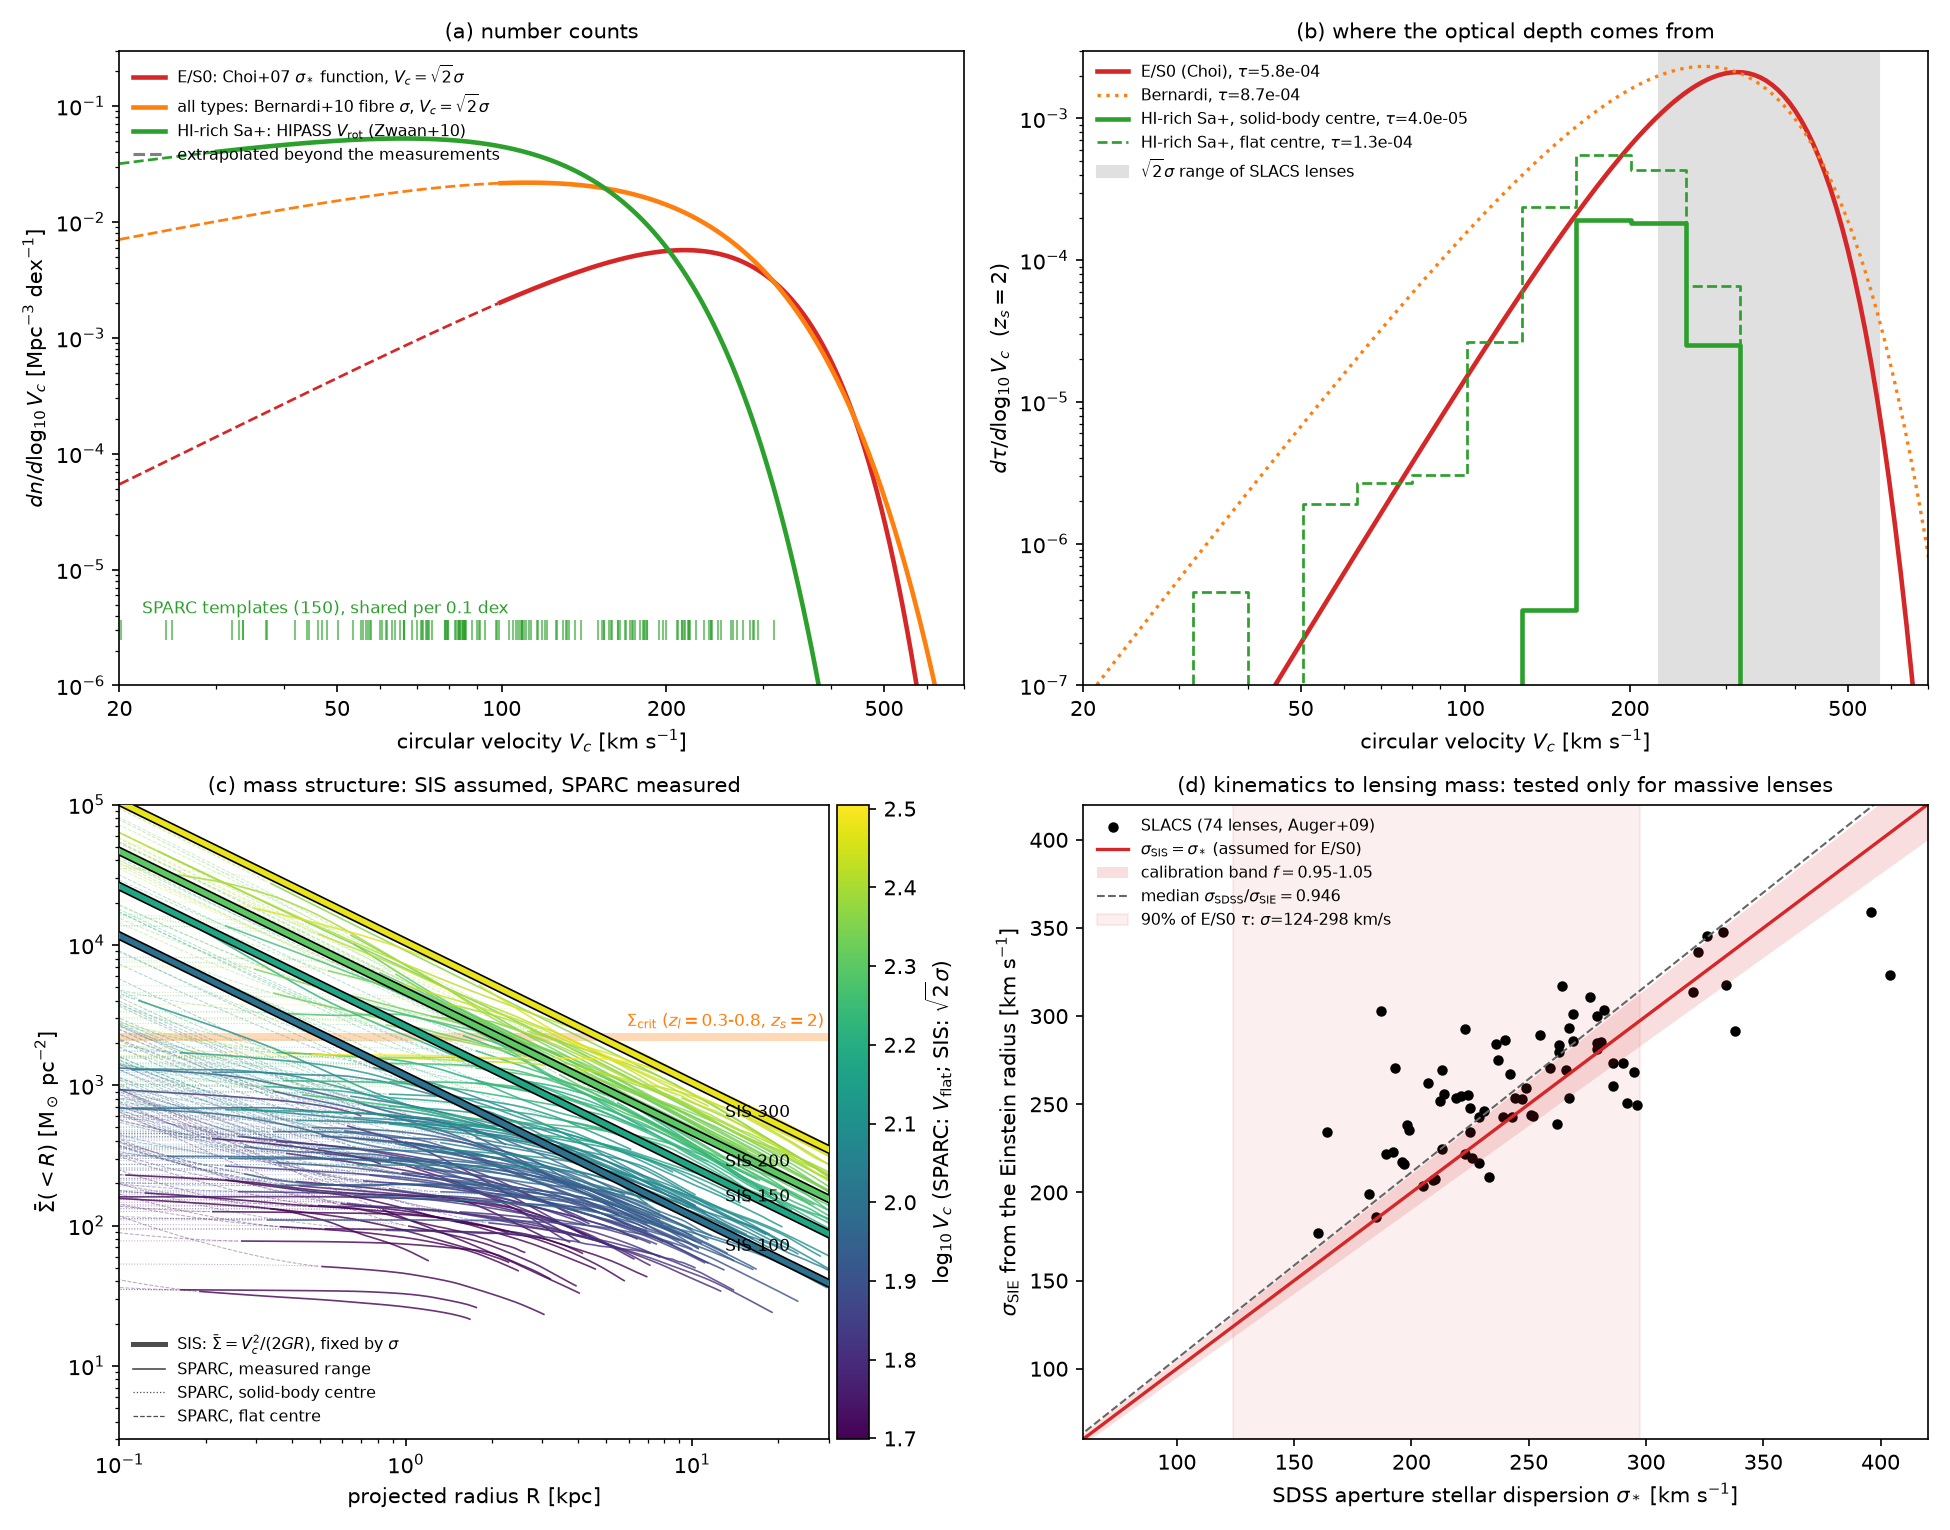
\includegraphics[width=\textwidth]{separations_compare_inputs.png}
\caption{Inputs. (a) Abundance per dex in circular velocity, solid where measured ($V_c=\sqrt2\sigma$ for the dispersion functions; the Bernardi et al.\ all-type function is shown for reference only). (b) Optical depth per dex in $V_c$: number times cross-section; grey marks the dispersions of SLACS lenses. (c) Mean projected density inside $R$: an SIS is fixed by $\sigma$ (outlined lines), SPARC galaxies are measured (thin lines; faint lines show the two inner extrapolations); the orange band is $\scrit$. (d) The SIS calibration: $\sigma_{\rm SIE}$ from the Einstein radius against the SDSS stellar dispersion for SLACS lenses; the pink band marks the dispersions that supply 90 per cent of the early-type optical depth.}
\label{fig:inputs}
\end{figure}

\section{Result}

\begin{figure}[t]
\centering
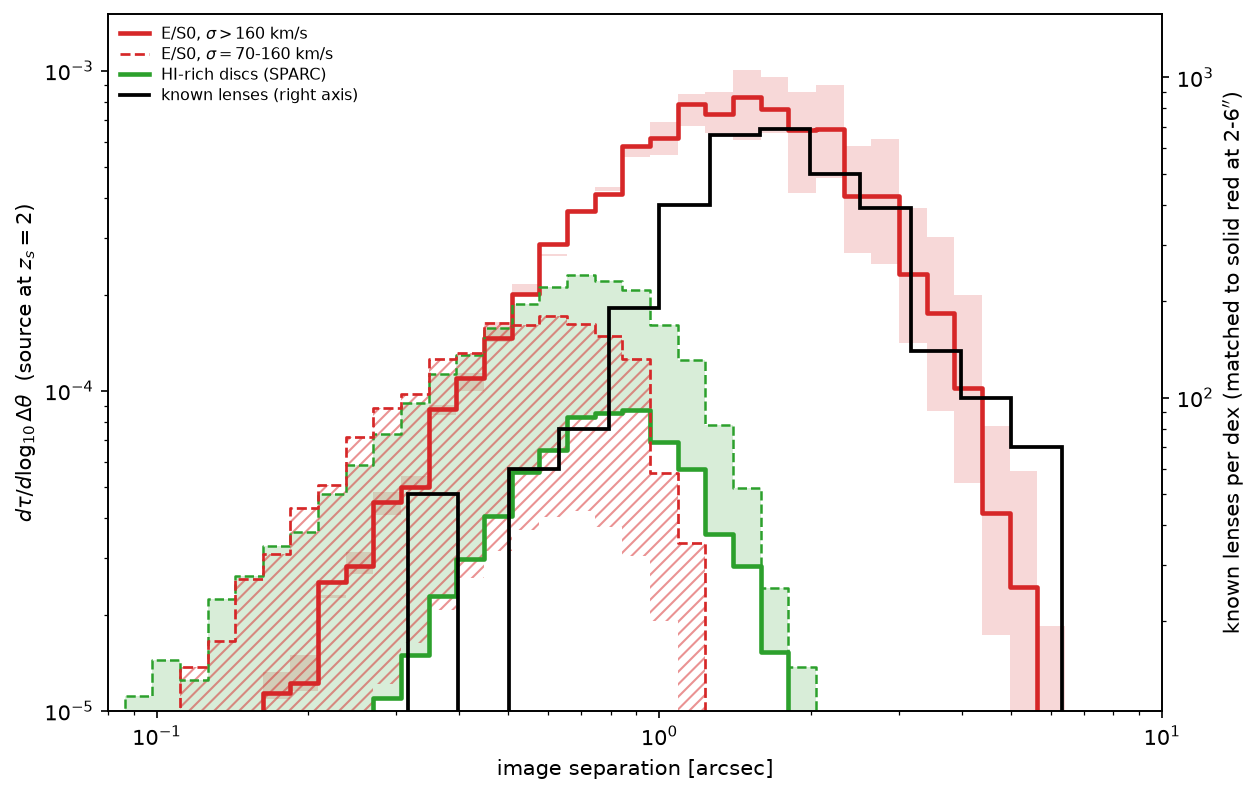
\includegraphics[width=0.85\textwidth]{separations_compare.png}
\caption{Image-separation distribution for a quasar at $z_s=2$, as optical depth per dex (left axis). Red solid: early types with $\sigma>160\kms$, counts \citep{Choi2007} and SIS mass calibration (SLACS) both measured; the band shows $\sigma_{\rm SIS}/\sigma_*=0.95$--$1.05$. Red dashed: early types with $\sigma=70$--$160\kms$, counted but with untested mass profiles, as SIS; the hatched band extends to an inner slope $\gamma=1.6$ inside $R_e=2$\,kpc (Section~\ref{sec:slope}). Green: HI-rich discs from SPARC rotation curves weighted by the HIPASS velocity function, with a solid-body (solid) or flat (dashed) centre inside the first measured point. Black: the 347 known lensed quasars of Gaia GraL~X \citep{Ducourant2026}, per dex (right axis), scaled to match the solid red curve at $2$--$6\arcsecond$. Non-evolving populations, spherical lenses, no magnification bias.}
\label{fig:result}
\end{figure}

\begin{table}[h]
\centering
\caption{Optical depth for a source at $z_s=2$.}
\label{tab:tau}
\begin{tabular}{lc}
\toprule
Population & $\tau$ \\
\midrule
E/S0, $\sigma>160\kms$ & $4.8\times10^{-4}$ \ ($4.0$--$5.9$ for $\sigma_{\rm SIS}/\sigma_*=0.95$--$1.05$) \\
E/S0, $\sigma=70$--$160\kms$ & $9.7\times10^{-5}$ \ (SIS; $2.0\times10^{-5}$ for $\gamma=1.6$) \\
HI-rich discs, solid-body centre & $4.0\times10^{-5}$ \ (flat centre: $1.3\times10^{-4}$) \\
\bottomrule
\end{tabular}
\end{table}

Figure~\ref{fig:result} shows the prediction; the two bands mark the two untested inputs, the inner profiles of intermediate-mass early types and of discs. Table~\ref{tab:sigma} breaks the early-type optical depth down by velocity dispersion in each separation range.

\begin{table}[h]
\centering
\caption{Share of the early-type optical depth by velocity dispersion, with lens-weighted medians.}
\label{tab:sigma}
\begin{tabular}{lcccccc}
\toprule
Separation & $\sigma<70$ & $70$--$160$ & $160$--$250$ & $>250$ & median $\sigma$ & median $z_l$ \\
\midrule
$0.1$--$0.5\arcsecond$ & 0.01 & 0.62 & 0.35 & 0.02 & $145\kms$ & 1.2 \\
$0.5$--$1\arcsecond$ & 0.00 & 0.28 & 0.66 & 0.06 & $179\kms$ & 0.9 \\
$1$--$2\arcsecond$ & 0.00 & 0.02 & 0.79 & 0.19 & $217\kms$ & 0.7 \\
$>2\arcsecond$ & 0.00 & 0.00 & 0.31 & 0.69 & -- & 0.5 \\
\bottomrule
\end{tabular}
\end{table}

\begin{enumerate}
\item \textbf{Above $1\arcsecond$ the prediction is anchored.} It comes from massive early types whose abundance and lensing mass are both measured.
\item \textbf{Sub-arcsecond lenses come by two routes.} Massive early types close to the source supply two-thirds of the $0.5$--$1\arcsecond$ lenses and a third of those below $0.5\arcsecond$ (median $z_l=0.9$ and 1.2). Early types with $\sigma=70$--$160\kms$ (median $145\kms$) supply 62 per cent below $0.5\arcsecond$ and 28 per cent at $0.5$--$1\arcsecond$, under the untested SIS assumption. With a shallower inner slope ($\gamma=1.6$, hatched band in Fig.~\ref{fig:result}) these fall to 21 and 9 per cent, and massive early types near the source dominate at all sub-arcsecond separations.
\item \textbf{Discs are a minority, dwarfs absent (spherical approximation).} Discs add 13 per cent of the lenses at $0.5$--$1\arcsecond$ and 9 per cent below $0.5\arcsecond$ (29 and 37 per cent with a flat centre, which is extrapolation). Of the 150 SPARC galaxies placed at $z_l=0.6$, only 31 lens, all with $V\geq126\kms$; the rest are subcritical according to their own rotation curves. Treating flattened discs as spheres is untested here: an edge-on disc concentrates its mass in projection and lenses more efficiently.
\end{enumerate}

\paragraph{Known lenses.} These are observed-to-predicted abundance ratios, not survey completeness: they assume the known sample is complete at $2$--$6\arcsecond$ and that the model predicts the relative abundances correctly, so the deficit mixes selection effects with model error. Scaled to the model at $2$--$6\arcsecond$, the known sample holds 175 lenses at $1$--$2\arcsecond$ against 252 predicted (0.7), 33 at $0.5$--$1\arcsecond$ against 107--173 (0.2--0.3), and 6 below $0.5\arcsecond$ against 31--89 (0.07--0.2). The ranges span the measured early types alone and all three components. Even counting only the measured early types, most sub-arcsecond lenses are missing.

\paragraph{Why not a halo model or an all-galaxy dispersion function.} Two alternatives give more sub-arcsecond lenses, and both fail the data. A halo model with NFW haloes, the \citet{Moster2013} stellar-to-halo relation and early-type sizes \citep{vanderWel2014} gives every halo a compact spheroid: at $V_c\approx130\kms$ its stars alone put $1.9\times10^9\,\msun$ inside 1\,kpc, against $5\times10^8\,\msun$ in total for SPARC galaxies of the same stellar mass and rotation speed. Coring the dark matter cannot close this gap, because the stars dominate the centre. For massive galaxies the same model is not isothermal: even with a Salpeter IMF and \citet{Cautun2020} contraction, which bring its total optical depth to that of the early types, it gives 1.45 times too many lenses at $0.3$--$1\arcsecond$ and 0.37 times too few at $2$--$4\arcsecond$. Without a galaxy, NFW haloes give $\tau\approx10^{-8}$. The all-type dispersion function of \citet{Bernardi2010} treated as SIS adds lenses below $1\arcsecond$ by assigning isothermal profiles to the bulge dispersions of discs, which SPARC shows to be far less concentrated.

\paragraph{Caveats.} \emph{Evolution.} The populations do not evolve, although the sub-arcsecond lenses sit at $z_l\approx0.9$--1.2. As an illustration, letting the early-type number density scale as $(1+z)^{-1}$ halves the optical depth below $1\arcsecond$ (0.48 below $0.5\arcsecond$, 0.54 at $0.5$--$1\arcsecond$, 0.69 at $2$--$6\arcsecond$), but changes the massive share only modestly (0.38 to 0.32 below $0.5\arcsecond$); a measured evolution of the velocity-dispersion function is the most important missing ingredient. \emph{Black holes.} A central black hole of $10^7$--$10^8\,\msun$, typical for $\sigma\approx100$--$160\kms$ \citep{Kormendy2013}, adds $\lesssim0.3$ per cent to the 0.8--$5\times10^{10}\,\msun$ inside the Einstein radius of these lenses and does not change the separations. \emph{Other.} Lenses are spherical, magnification bias is not applied, and the source redshift is fixed at $z_s=2$.

\section{Sensitivity to the central slope}\label{sec:slope}

The intermediate early types are the uncertain ingredient, so we replace their SIS profiles by $\rho\propto r^{-\gamma}$ inside $R_e$ and isothermal outside, normalised so that the mass inside $R_e$ equals the SIS value $2\sigma^2R_e/G$, the mass the stellar dispersion measures. $\gamma=2$ recovers the SIS. Because profiles with $\gamma>2$ have divergent central deflections and formally image every source through vanishingly faint counter-images, we count a source as lensed only if the fainter outer image has at least 10 per cent of the brighter one's flux, the range of the QUELLS calibration grid; this is applied to all variants, including the massive early types.

\begin{figure}[t]
\centering
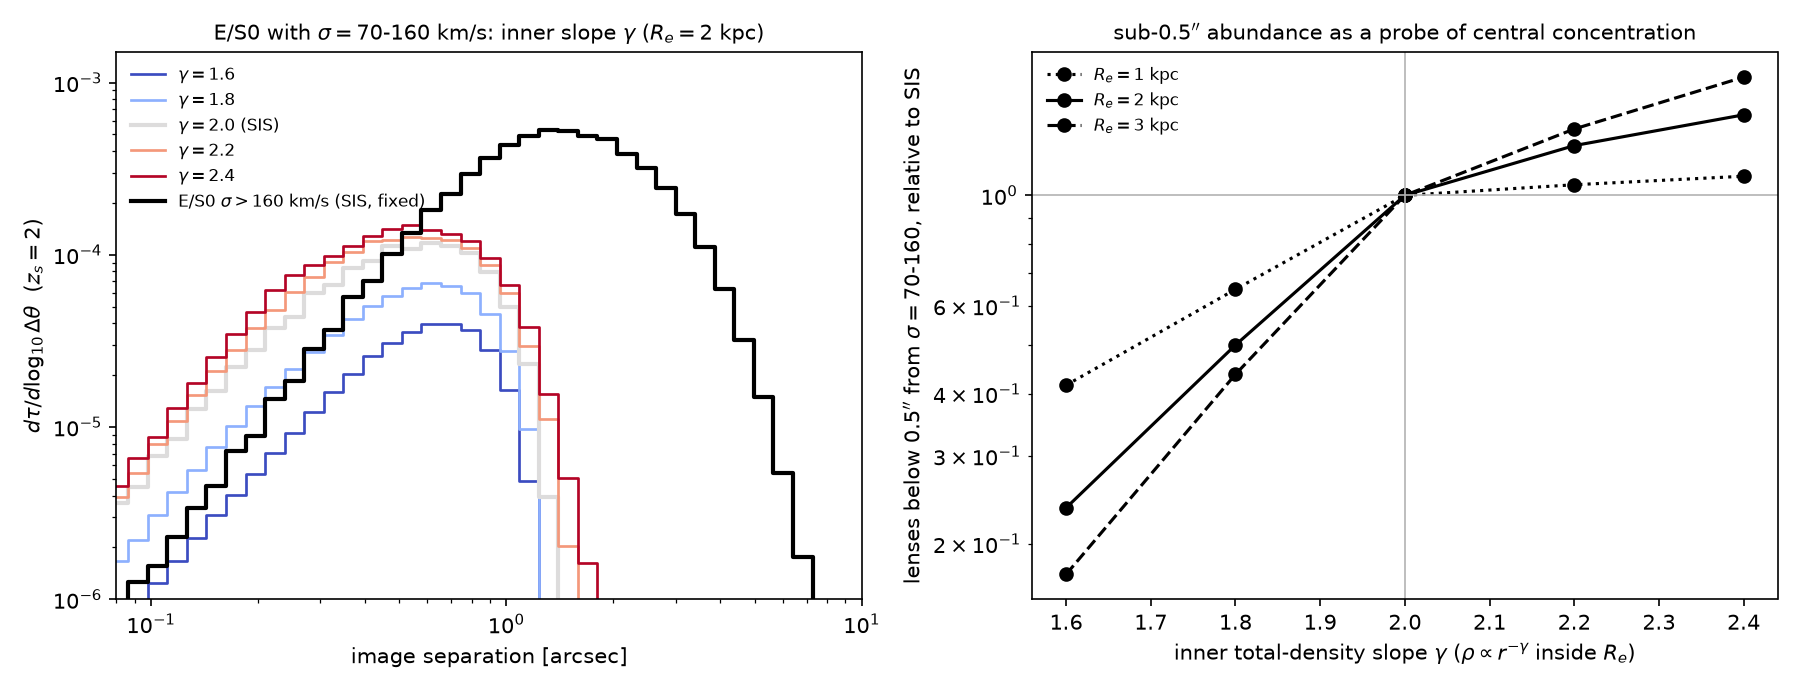
\includegraphics[width=\textwidth]{slope_test.png}
\caption{Left: separation distribution of early types with $\sigma=70$--$160\kms$ for inner slopes $\gamma=1.6$--2.4 ($R_e=2$\,kpc), with the massive early types fixed (black). Right: their optical depth below $0.5\arcsecond$ relative to the SIS, for $R_e=1$, 2 and 3\,kpc. Flux ratio of the two outer images $\geq0.1$.}
\label{fig:slope}
\end{figure}

The response is strong and asymmetric (Fig.~\ref{fig:slope}). For $R_e=2$\,kpc, shallower centres remove most of the sub-$0.5\arcsecond$ lenses from these galaxies (0.50 of the SIS value at $\gamma=1.8$, 0.24 at 1.6), and their share of all early-type lenses below $0.5\arcsecond$ falls from 0.62 to 0.28. Steeper centres raise it only modestly (1.26 at $\gamma=2.2$, 1.45 at 2.4), because the extra central mass mostly feeds faint central images. Larger sizes strengthen the response ($\times0.17$ at $\gamma=1.6$ for $R_e=3$\,kpc) and smaller ones weaken it ($\times0.42$ for 1\,kpc). At $0.5$--$1\arcsecond$ the share falls from 0.30 to 0.13 at $\gamma=1.6$.

\section{Time delays}
\label{sec:delays}

QUELLS measures time delays from unresolved light curves; this is its defining capability, and it turns the separation distribution into a joint distribution of separations and delays.

\paragraph{Mass versus potential.} Image positions and delays measure different things. Positions follow from the lens equation $\boldsymbol\beta=\boldsymbol\theta-\boldsymbol\alpha(\boldsymbol\theta)$ with $\boldsymbol\alpha=\nabla\psi$, the gradient of the projected potential; for a circular lens this fixes the mass enclosed within the Einstein radius,
\begin{equation}
M_{\rm 2D}(<R_E)=\pi R_E^2\,\scrit ,
\end{equation}
but not how that mass is distributed: power laws $\rho\propto r^{-\gamma}$ with different $\gamma$ give the same $\theta_E$ once renormalised. The delay depends on the potential itself,
\begin{equation}
\Delta t_{AB}=\frac{D_{\Delta t}}{c}\left[\phi(\boldsymbol\theta_B)-\phi(\boldsymbol\theta_A)\right],\qquad
\phi(\boldsymbol\theta)=\tfrac12|\boldsymbol\theta-\boldsymbol\beta|^2-\psi(\boldsymbol\theta),\qquad
\nabla^2\psi=2\kappa ,
\end{equation}
so it integrates the mass between the images. For a circular lens and images near the Einstein radius, at fixed image positions, cosmology and redshifts, $\Delta t\propto1-\langle\kappa\rangle$, the mean convergence in the annulus between the images \citep{Kochanek2002}. A power law normalised to the same $\theta_E$ has $\kappa(\theta_E)=(3-\gamma)/2$, which gives
\begin{equation}
\Delta t=\frac{D_{\Delta t}}{2c}\left(\theta_A^2-\theta_B^2\right)(\gamma-1).
\end{equation}
Our lensing code reproduces this to three decimals for $\gamma=1.6$--2.4:

\begin{center}
\begin{tabular}{lccccc}
\toprule
$\gamma$ & 1.6 & 1.8 & 2.0 & 2.2 & 2.4 \\
$\kappa(\theta_E)$ & 0.70 & 0.60 & 0.50 & 0.40 & 0.30 \\
delay relative to SIS, same images & 0.6 & 0.8 & 1.0 & 1.2 & 1.4 \\
\bottomrule
\end{tabular}
\end{center}

More concentrated profiles put less mass in the annulus and give longer delays. The response has a known limit: the mass-sheet transformation
\begin{equation}
\kappa\to\lambda\kappa+(1-\lambda)
\end{equation}
leaves the image positions unchanged and rescales the delay by $\lambda$ at fixed $D_{\Delta t}$, so a single delay does not fix both the profile and the distance \citep{Sonnenfeld2018}. With cosmology fixed externally, the delay constrains the profile up to this degeneracy, which lens redshifts, stellar kinematics and the population's measured abundances help to break.

\paragraph{Delays of the predicted population.} We compute the delay between the two outer images from the Fermat potential, $\Delta t=(D_{\Delta t}/c)\,\Delta\phi$ with $\phi=\tfrac12(\theta-\beta)^2-\psi$, $\psi=\int\alpha\,d\theta$ and $D_{\Delta t}=(1+z_l)D_lD_s/D_{ls}$, for the same populations, counting sources whose fainter image has at least 10 per cent of the brighter one's flux. The SIS delays reproduce $\Delta t=(D_{\Delta t}/2c)\,\Delta\theta^2(1-q)/(1+q)$ to 1.5 per cent.

\begin{figure}[t]
\centering
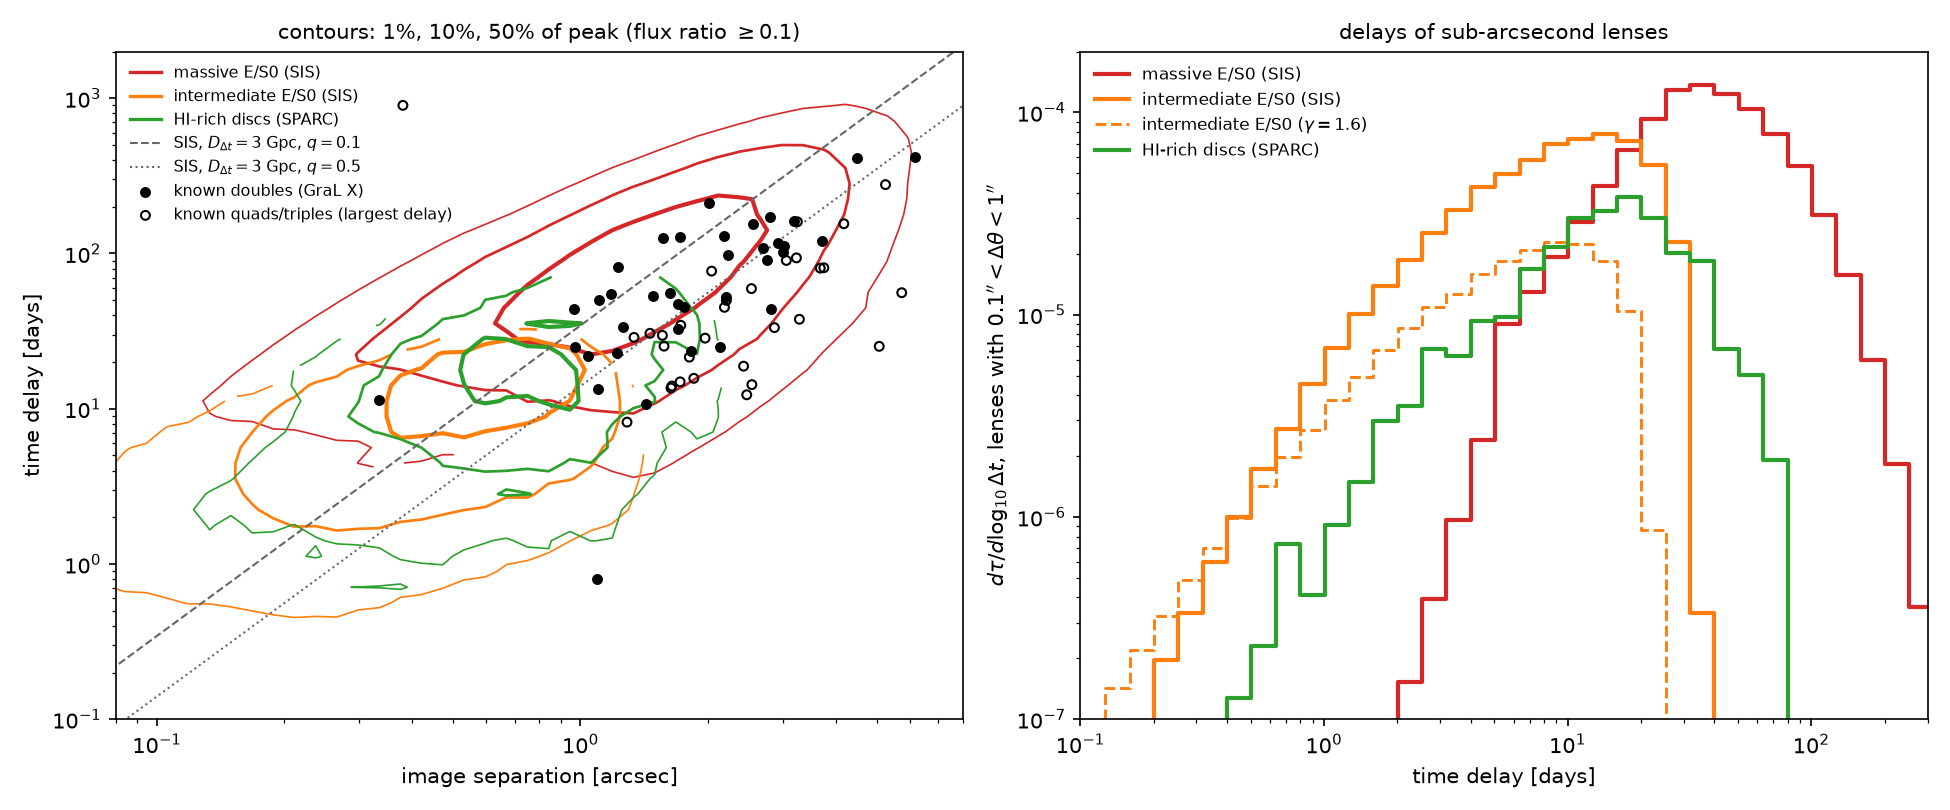
\includegraphics[width=\textwidth]{delays.png}
\caption{Left: joint distribution of image separation and time delay for a source at $z_s=2$ (contours at 1, 10 and 50 per cent of each population's peak; flux ratio $\geq0.1$). Lines: SIS relation for $D_{\Delta t}=3$\,Gpc and $q=0.1$ (dashed) or 0.5 (dotted). Points: the 68 known lenses with measured delays (GraL~X; filled doubles, open quads and triples with their largest delay). Right: delay distributions of lenses with $0.1<\Delta\theta<1\arcsecond$.}
\label{fig:delays}
\end{figure}

\begin{table}[h]
\centering
\caption{Median time delay and, in brackets, the share of lenses with delays of 10--120\,d, where QUELLS recovers at least about half of the delays from ZTF sampling; all sub-arcsecond lenses have delays below 120\,d. Flux ratio $\geq0.1$, $z_s=2$.}
\label{tab:delays}
\begin{tabular}{lccc}
\toprule
Population & $0.1$--$0.5\arcsecond$ & $0.5$--$1\arcsecond$ & $1$--$2\arcsecond$ \\
\midrule
E/S0, $\sigma>160\kms$ & 21\,d (0.89) & 36\,d (0.94) & 60\,d (0.78) \\
E/S0, $\sigma=70$--$160\kms$, SIS & 6\,d (0.31) & 11\,d (0.63) & -- \\
E/S0, $\sigma=70$--$160\kms$, $\gamma=1.6$ & 3.5\,d (0.10) & 7.7\,d (0.40) & -- \\
HI-rich discs & 9\,d (0.52) & 15\,d (0.76) & 24\,d (0.85) \\
\bottomrule
\end{tabular}
\end{table}

Three results follow (Fig.~\ref{fig:delays}, Table~\ref{tab:delays}).
\begin{enumerate}
\item \textbf{The delay identifies the route.} At the same separation, massive deflectors near the source have delays three to four times longer than intermediate-mass ones, because their time-delay distance is larger. Separation and delay together therefore classify a lens without a deflector redshift, which is hard to obtain for a faint galaxy next to bright quasar images.
\item \textbf{The delay responds to the inner slope.} A $\gamma=1.6$ lens has a 40 per cent shorter delay than an isothermal lens with the same images, so shallower centres give both fewer sub-arcsecond lenses and shorter delays (median 3.5 instead of 6\,d below $0.5\arcsecond$). Because of the mass-sheet degeneracy the constraint is statistical, on the slope distribution of the population, rather than from individual doubles.
\item \textbf{The selection function in delay matters.} All sub-arcsecond lenses have delays below the $\sim120$\,d limit set by ZTF's seasonal gaps, so all are within reach; what differs is the efficiency at short delays. About 90 per cent of massive deflectors near the source have delays above 10\,d, where the paper's injections recover at least half of them, against 31 per cent of intermediate-mass ones below $0.5\arcsecond$ (63 per cent at $0.5$--$1\arcsecond$), and only 10 per cent if their centres are shallow ($\gamma=1.6$). Shallow centres therefore also make the lenses harder to recover. The intermediate-mass test needs the QUELLS detection efficiency measured as a function of delay down to a few days, which the injection framework can do, and benefits from denser cadence such as Rubin's.
\end{enumerate}
The known lenses with measured delays lie on the locus of massive early types, as the model predicts for systems wider than $1\arcsecond$.

\section{What sub-arcsecond lenses can measure}

Lensing measures projected mass directly, independent of stellar populations and dynamical modelling, but until now it has done so almost only for massive galaxies: SLACS lenses have $\sigma\gtrsim160\kms$, and SLACS and SL2S deflectors have $M_*\gtrsim10^{10.5}\,\msun$. Sub-arcsecond lenses reach below this. In our prediction they are the one population in which galaxies of $\sigma\approx100$--$160\kms$ dominate the lensing, and in that regime the central mass profile is unconstrained: an isothermal centre, as observed for massive early types, puts $4\times10^9\,\msun$ inside 1\,kpc at $V_c=130\kms$, eight times the mass measured there in SPARC discs of the same rotation speed.

The sharpest form of the claim is therefore: \emph{sub-arcsecond lenses test whether the near-isothermal total mass profiles of massive early-type lenses extend to intermediate-mass galaxies with $\sigma\approx70$--$160\kms$.} This is a measurement in three ways.
\begin{itemize}
\item \textbf{Abundance.} If galaxies with $\sigma\approx100$--$160\kms$ are isothermal, they supply most lenses below $0.5\arcsecond$; if they are less concentrated, those lenses become rarer and come mainly from massive galaxies near the source. The number of sub-arcsecond lenses in a sample with a known selection function therefore constrains the central concentration of intermediate-mass galaxies as a population. The counts of these galaxies are already measured \citep{Choi2007}, so their lensing efficiency is the only unknown. A shallower slope, $\gamma=1.6$ rather than 2, would remove three-quarters of their sub-$0.5\arcsecond$ lenses (Fig.~\ref{fig:slope}).
\item \textbf{Delays.} The joint distribution of separations and delays responds to the inner slope twice: shallower centres give fewer sub-arcsecond lenses and shorter delays at fixed image positions ($\Delta t\propto\gamma-1$). Fitting this joint distribution, with the selection function measured by injection, constrains the slope distribution of intermediate-mass galaxies at the population level. The mass-sheet degeneracy still limits individual doubles; the measured abundances, lens redshifts and stellar kinematics are what break it. At fixed separation the delay also separates massive deflectors near the source from intermediate-mass ones.
\item \textbf{Individual systems.} With a deflector redshift, which separates the two routes because $\Delta\theta\propto\sigma^2D_{ls}/D_s$, each lens gives the projected mass inside a radius of 1--3\,kpc. Combined with stellar mass and, where possible, stellar kinematics, this yields dark-matter fractions and total density slopes for intermediate-mass galaxies, the regime where stellar feedback and the stellar IMF are expected to change most and where SLACS-like constraints do not exist.
\end{itemize}
Massive deflectors at $z_l\approx1$ add a second benefit: they extend the lensing measurement of massive-galaxy structure to earlier times.

The same framework connects directly to galaxy-formation simulations. Rather than comparing dark-matter responses alone, each simulation predicts the joint distribution of stellar mass, size, total inner slope and dark-matter fraction within a fixed aperture as a function of halo mass and redshift; propagating it through the lensing calculation gives $d\tau/d\log\Delta\theta$. Feedback, the stellar IMF and dark-matter contraction then enter through the quantity the lenses measure, the central total mass profile, and Fig.~\ref{fig:slope} shows how accurately the simulations must predict it to be tested.

QUELLS selects lenses by variability rather than morphology and measures their delays from the blended light curve, so its selection function does not depend on whether the images are resolved, and it can be calibrated by injection as a function of separation, delay and flux ratio. That is what both the abundance test and the delay test require. Time-delay cosmography with this population is possible in principle, but compact doubles with faint deflectors constrain the lens potential weakly; we regard it as secondary to the galaxy-structure measurement.

\begin{thebibliography}{99}
\bibitem[Auger et al.(2009)]{Auger2009} Auger M. W., et al., 2009, ApJ, 705, 1099, arXiv:0911.2471
\bibitem[Bernardi et al.(2010)]{Bernardi2010} Bernardi M., et al., 2010, MNRAS, 404, 2087, arXiv:0910.1093
\bibitem[Bolton et al.(2008)]{Bolton2008} Bolton A. S., et al., 2008, ApJ, 684, 248, arXiv:0805.1932
\bibitem[Cautun et al.(2020)]{Cautun2020} Cautun M., et al., 2020, MNRAS, 494, 4291, arXiv:1911.04557
\bibitem[Choi et al.(2007)]{Choi2007} Choi Y.-Y., Park C., Vogeley M. S., 2007, ApJ, 658, 884, arXiv:astro-ph/0611607
\bibitem[Ducourant et al.(2026)]{Ducourant2026} Ducourant C., et al., 2026, A\&A, 707, A345, arXiv:2603.12810
\bibitem[Kormendy \& Ho(2013)]{Kormendy2013} Kormendy J., Ho L. C., 2013, ARA\&A, 51, 511, arXiv:1304.7762
\bibitem[Kochanek(2002)]{Kochanek2002} Kochanek C. S., 2002, ApJ, 578, 25, arXiv:astro-ph/0205319
\bibitem[Lelli et al.(2016)]{Lelli2016} Lelli F., McGaugh S. S., Schombert J. M., 2016, AJ, 152, 157, arXiv:1606.09251
\bibitem[Moster et al.(2013)]{Moster2013} Moster B. P., Naab T., White S. D. M., 2013, MNRAS, 428, 3121, arXiv:1205.5807
\bibitem[Sonnenfeld(2018)]{Sonnenfeld2018} Sonnenfeld A., 2018, MNRAS, 474, 4648
\bibitem[van der Wel et al.(2014)]{vanderWel2014} van der Wel A., et al., 2014, ApJ, 788, 28, arXiv:1404.2844
\bibitem[Zwaan et al.(2010)]{Zwaan2010} Zwaan M. A., Meyer M. J., Staveley-Smith L., 2010, MNRAS, 403, 1969, arXiv:0912.1754
\end{thebibliography}

\end{document}
